\section{Empirical Results}
\vspace{-3mm}

\textbf{Models.}
We evaluate \textsc{Didr} on two backbones. For primary experiments, we apply \textsc{Didr} to one-step SDXL~\citep{podell2023sdxl} at $1024\times1024$ resolution, initializing the generator from the DMD2-SDXL-1step checkpoint~\citep{yin2024improved} and using the pretrained SDXL diffusion model as both the frozen reference $s_{\mathrm{ref}}$ and the TA initialization. We report a standard variant (\textsc{Didr}) and an extended-training variant (\textsc{Didr}$_{\text{longer}}$). To assess generalizability, we additionally apply \textsc{Didr} to the Z-Image backbone~\citep{zimage} (\textsc{zimage-Didr}), initializing from Z-Image-Turbo. Full hyperparameters are in Appendix~\ref{app:implementation}.

\textbf{Training Data and Reward.}
All models are trained on text prompts from LAION-Aesthetic-6.25+~\citep{zhou2024long}; no image data is required. As the reward model $r(x_0,c)$, we use PickScore~\citep{pickscore}, a widely accepted human preference model trained on large-scale pairwise human annotations that scores how well a generated image matches human preference given a text prompt. The training reward uses the raw unscaled PickScore, which is $1/98.86$ of the official reported values in Table~\ref{tab:main}, making $\tau{=}0.01$ a reasonable temperature for the DRP softmax.

\textbf{Evaluation.}
We report three categories of metrics: \textit{Preference} --- PickScore~\citep{pickscore}, ImageReward~\citep{xu2023imagereward}, HPSv2.1~\citep{hpsv2}, and Aesthetic Score~\citep{laionaes}; \textit{Text alignment} --- CLIPScore~\citep{hessel2021clipscore,radford2021learning}, DPG-Bench~\citep{dpgbench}, and GenEval~\citep{geneval}; and \textit{Fidelity} --- FID~\citep{heusel2017gans}. PickScore, ImageReward, Aesthetic Score, and CLIPScore are evaluated on $1\text{k}$ prompts from the MSCOCO-2017 validation set~\citep{lin2014microsoft}; FID on the full $30\text{k}$ validation images; HPSv2.1, DPG-Bench, and GenEval each use their own standard benchmark prompts. Since PickScore is also our training reward, the remaining preference metrics serve as independent out-of-domain evaluations. Further details are provided in Appendix~\ref{app:evaluation_metrics}.

\vspace{-3mm}
\subsection{Quantitative Results}

\textbf{\textsc{Didr}$_{\text{longer}}$ achieves the highest PickScore among evaluated one-step text-to-image models.}
As shown in Table~\ref{tab:main}, \textsc{Didr}$_{\text{longer}}$ achieves the highest PickScore ($23.9$) and surpasses all multi-step reference models on all four preference metrics under our evaluation protocol, using only 2.6B parameters and a single inference step. Gains span both the training reward and independent out-of-domain metrics (ImageReward $+8.9\%$, HPSv2.1 $+0.6$, Aesthetic Score $+0.15$ over DI*), suggesting that alignment does not simply overfit to PickScore. Per-category GenEval and HPSv2.1 results are provided in Tables~\ref{tab:geneval} and~\ref{tab:hpsv2} (Appendix~\ref{app:geneval}).

\textbf{Standard \textsc{Didr} Pareto-dominates all one-step alignment baselines on preference vs.\ fidelity.}
\begin{figure}[!t]
\centering
\begin{subfigure}[b]{0.48\linewidth}
  \centering
  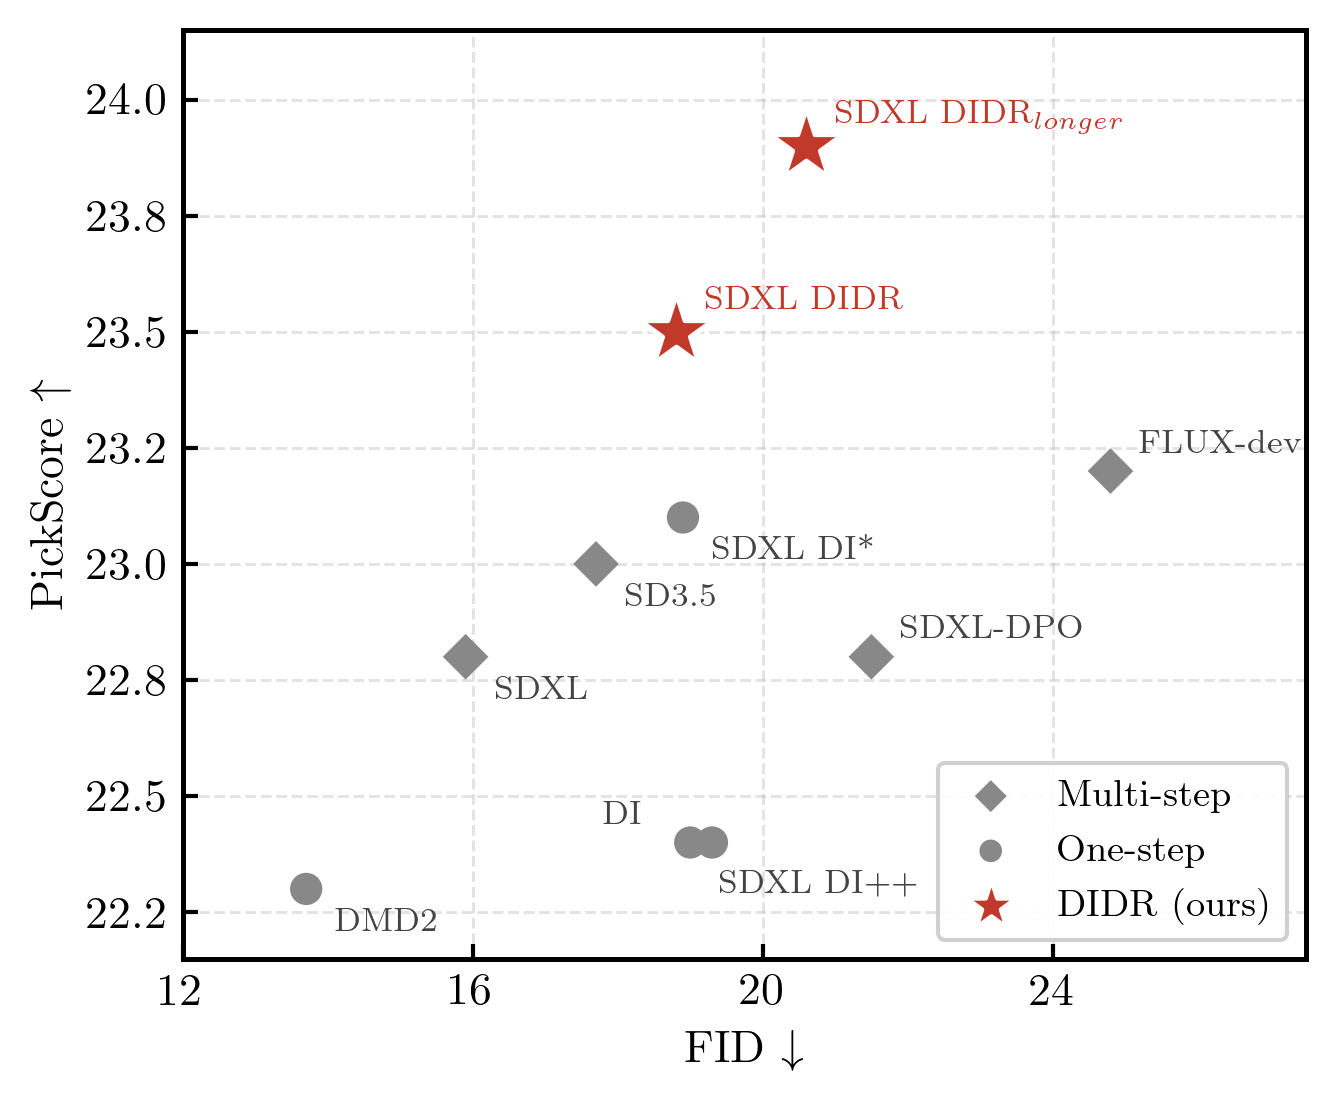
\includegraphics[width=0.85\linewidth]{pictures/model_scatter.png}
  \phantomcaption
  \label{fig:pareto}
\end{subfigure}
\hfill
\begin{subfigure}[b]{0.48\linewidth}
  \centering
  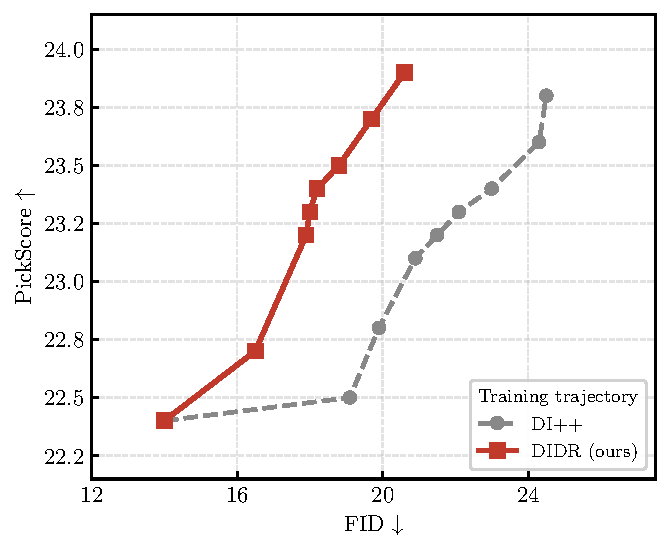
\includegraphics[width=0.85\linewidth]{pictures/training_trajectory.pdf}
  \phantomcaption
  \label{fig:trajectory}
\end{subfigure}
\caption{\textbf{PickScore--FID analysis}. \textit{Left}: final model comparison on MSCOCO-2017; \textsc{Didr} Pareto-dominates all one-step alignment baselines. \textit{Right}: training trajectories, \textsc{Didr} vs.\ Diff-Instruct++.}
\label{fig:pickscore_fid}
\vspace{-0.1in}
\end{figure}
Since the target distribution is the reward-tilted $q^*$ (Eq.~\eqref{eq:reward_tilted_target}), some FID increase is theoretically expected; the key question is which method best navigates this trade-off. As shown in Figure~\ref{fig:pareto}, \textsc{Didr} (PickScore $23.5$, FID $18.8$) Pareto-dominates all one-step alignment baselines and simultaneously surpasses FLUX-dev and SDXL-DPO on both axes. \textsc{Didr} also maintains text alignment, achieving the highest DPG-Bench ($75.06$) and GenEval ($0.579$) among one-step SDXL methods, with only a marginal CLIPScore dip, which is expected since text-alignment metrics are not directly optimized by the reward model.

\textbf{\textsc{Didr} generalizes across architectures and model scales.}
\textsc{Didr} generalizes to DiT architectures at larger scale: applied to the 6B-parameter Z-Image backbone, \textsc{zimage-Didr} surpasses the 50-step Z-Image base on all preference metrics in a single step. Against the 8-step Z-Image-Turbo, it leads on ImageReward, Aesthetic Score, CLIPScore, and DPG-Bench with lower FID, while trailing on PickScore, HPSv2.1, and GenEval. These gains are driven by training, not initialization---the 1-step Z-Image-Turbo initially scores ImageReward $0.39$ and FID $36.7$, vs $1.08$ and $22.1$ for \textsc{zimage-Didr}.

\begin{table*}[!t]
\centering
\caption{Comparison of \textsc{Didr} against baselines at $1024\times1024$ resolution. Multi-step models are shown as reference only (no bold). \textbf{Bold}: best result within each one-step group. $\uparrow$/$\downarrow$: higher/lower is better. $^\dagger$: Z-Image-Turbo at 1~NFE (unofficial; \textsc{Didr} training initialization only).}
\label{tab:main}
\resizebox{\textwidth}{!}{\begin{tabular}{lclccccccccc}
\toprule
& & & & \multicolumn{4}{c}{\textbf{Preference} $\uparrow$} & \multicolumn{3}{c}{\textbf{Text Alignment} $\uparrow$} & \\
\cmidrule(lr){5-8} \cmidrule(lr){9-11}
\textbf{Model} & \textbf{Steps} & \textbf{Arch.} & \textbf{Params} & \textbf{PickS.} & \textbf{ImgR.} & \textbf{HPSv2.1} & \textbf{Aesth.} & \textbf{CLIP} & \textbf{DPG} & \textbf{GenEval} & \textbf{FID} $\downarrow$ \\
\midrule
\multicolumn{12}{l}{\textit{Multi-step reference}} \\
SDXL~\citep{podell2023sdxl}            & 50 & UNet & 2.6B & 22.8 & 0.82 & 28.98 & 5.45 & 33.86 & 74.42 & 0.551 & 15.9 \\
SDXL-DPO~\citep{wallace2024diffusion}  & 50 & UNet & 2.6B & 22.8 & 0.92 & 30.45 & 5.61 & 33.97 & 74.24 & 0.549 & 21.5 \\
SD3.5-large~\citep{sd35}               & 28 & DiT  & 8B   & 23.0 & 1.01 & 30.06 & 5.42 & 33.85 & 84.88 & 0.717 & 17.7 \\
FLUX-dev~\citep{fluxdev}               & 50 & DiT  & 12B  & 23.2 & 1.05 & 30.65 & 5.54 & 32.88 & 83.86 & 0.672 & 24.8 \\
Z-Image~\citep{zimage}                 & 50 & DiT  & 6B   & 22.5 & 0.99 & 30.57 & 5.43 & 33.15 & 86.30 & 0.840 & 14.3 \\
\midrule
\multicolumn{12}{l}{\textit{One-step SDXL}} \\
SDXL DMD2~\citep{yin2024improved}                  & 1 & UNet & 2.6B & 22.3 & 0.83 & 29.99 & 5.47 & 33.31 & 74.01 & 0.557 & \textbf{13.7} \\
SDXL Diff-Instruct~\citep{Luo2023DiffInstructAU}   & 1 & UNet & 2.6B & 22.4 & 0.92 & 31.51 & 5.53 & 33.35 & 74.98 & 0.560 & 19.3 \\
SDXL Diff-Instruct++~\citep{anonymous2024diffinstruct} & 1 & UNet & 2.6B & 22.4 & 0.92 & 31.44 & 5.58 & \textbf{33.37} & 75.01 & 0.560 & 19.0 \\
SDXL Diff-Instruct*~\citep{luo2024onestep}          & 1 & UNet & 2.6B & 23.1 & 1.01 & 33.29 & 5.68 & 33.09 & 74.97 & 0.555 & 18.9 \\
\textbf{SDXL \textsc{Didr} (Ours)}                  & 1 & UNet & 2.6B & 23.5 & 1.04 & 33.77 & 5.82 & 33.03 & \textbf{75.06} & \textbf{0.579} & 18.8 \\
\textbf{SDXL \textsc{Didr}$_{\text{longer}}$ (Ours)} & 1 & UNet & 2.6B & \textbf{23.9} & \textbf{1.10} & \textbf{33.89} & \textbf{5.83} & 32.97 & 74.99 & 0.566 & 20.6 \\
\midrule
\multicolumn{12}{l}{\textit{Z-Image backbone}} \\
Z-Image-Turbo~\citep{zimage}                        & 8 & DiT & 6B & \textbf{23.0} & 1.01 & \textbf{31.86} & 5.39 & 33.08 & 85.00 & \textbf{0.750} & 25.2 \\
\textbf{Z-Image \textsc{Didr} (Ours)}               & 1 & DiT & 6B & 22.6 & \textbf{1.08} & 31.40 & \textbf{5.46} & \textbf{33.35} & \textbf{86.63} & 0.692 & \textbf{22.1} \\
\hdashline
Z-Image-Turbo$^\dagger$~\citep{zimage}              & 1 & DiT & 6B & 21.0 & 0.39 & 24.54 & 4.68 & 33.28 & 77.05 & 0.572 & 36.7 \\
\bottomrule
\end{tabular}}
\vspace{-0.15in}
\end{table*}


\vspace{-3mm}
\subsection{Qualitative Comparison}
\vspace{-3mm}

\begin{figure}[!t]
\centering
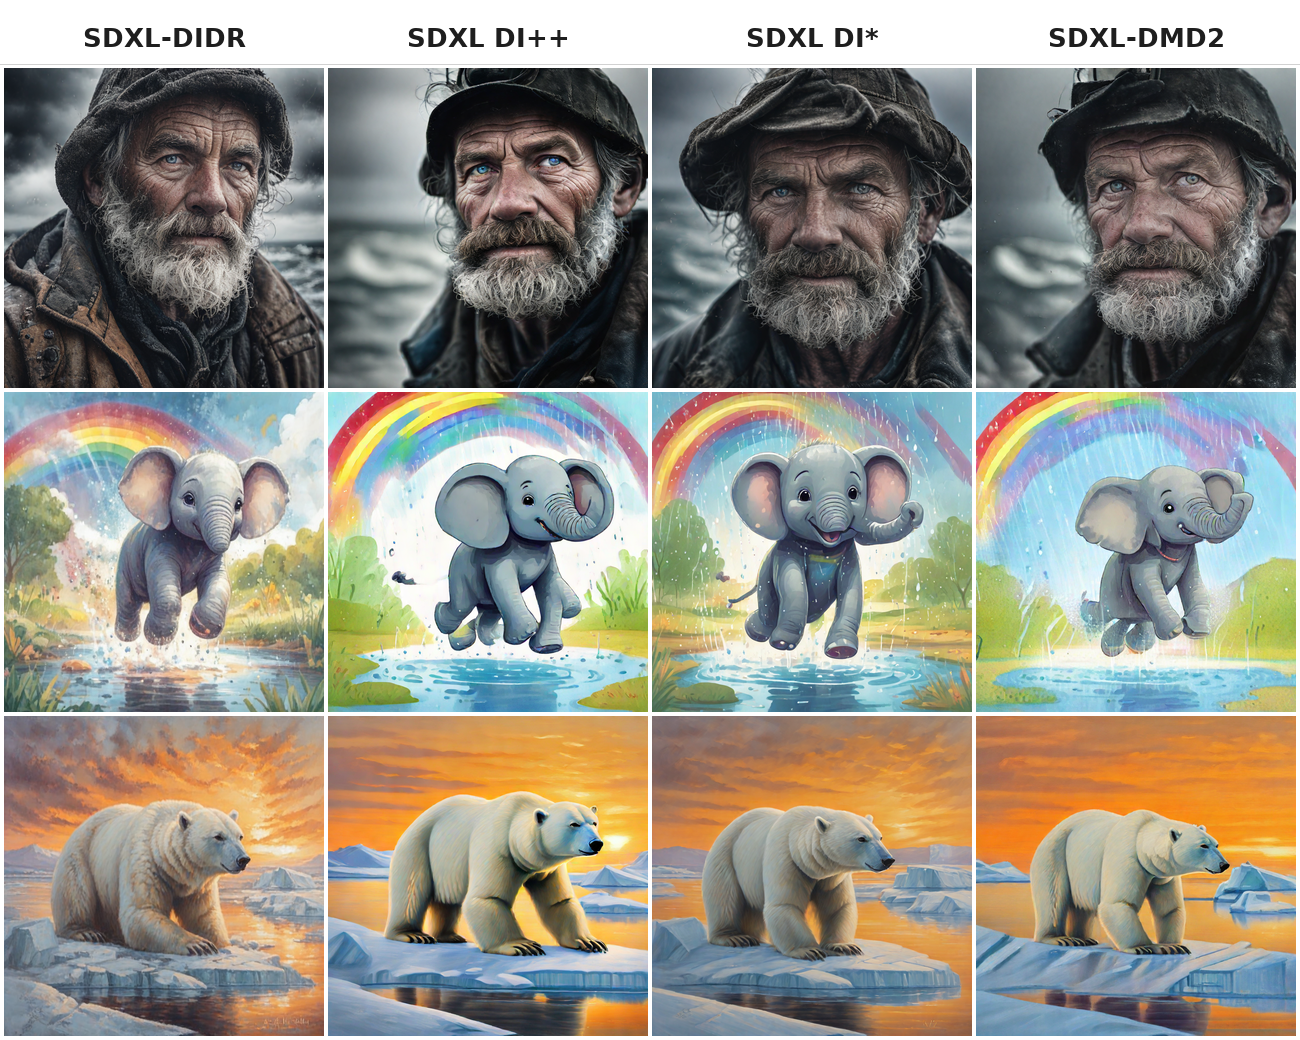
\includegraphics[width=0.571\textwidth]{pictures/comparison_sdxl.png}
\hfill
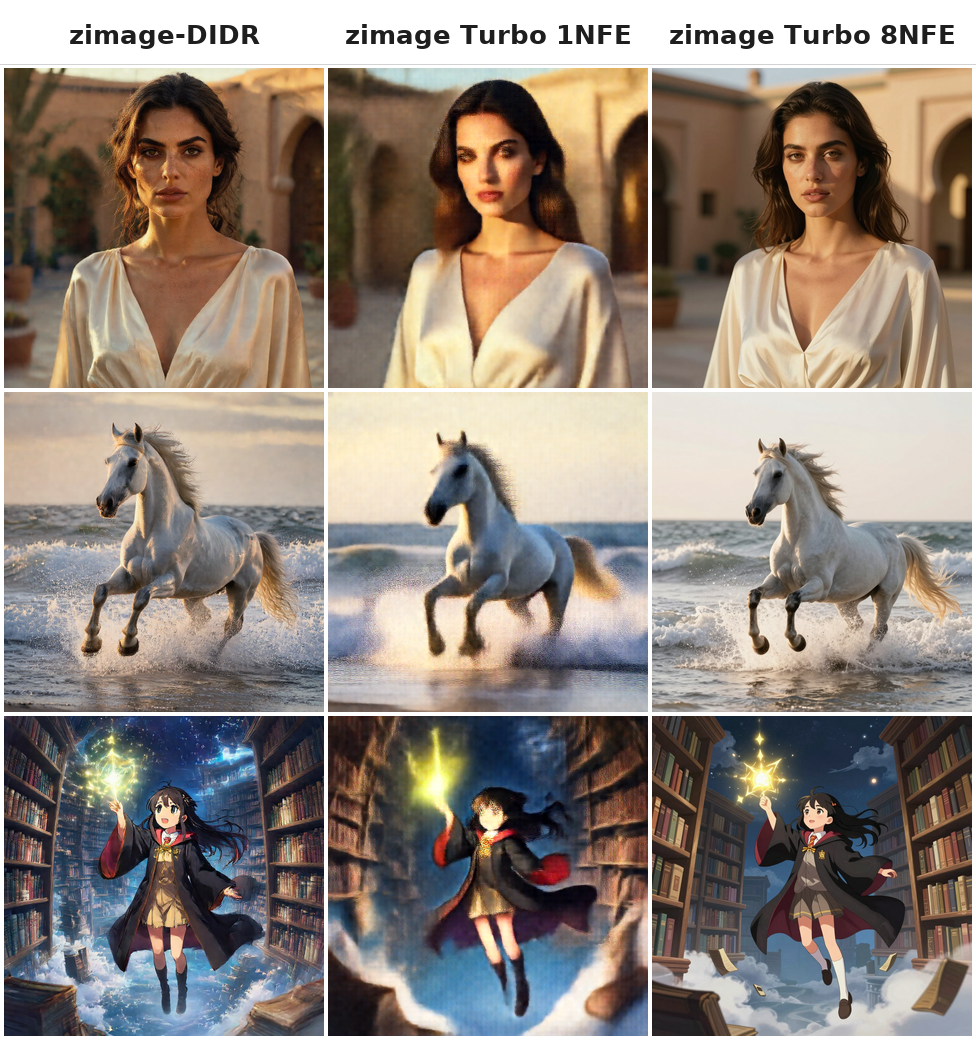
\includegraphics[width=0.428\textwidth]{pictures/comparison_zimage.png}
\caption{\textbf{Qualitative comparison at $1024\times1024$.} \textit{Left}: SDXL backbone (SDXL-DIDR, DI++, DI*, DMD2). \textit{Right}: Z-Image backbone (zimage-DIDR, Turbo 1NFE, Turbo 8NFE). Rows: backbone-specific prompts listed in Appendix~\ref{app:prompts}.}
\label{fig:qualitative}
\vspace{-0.1in}
\end{figure}

\textsc{Didr} consistently improves visual quality over prior one-step methods while preserving perceptual naturalness (Figures~\ref{fig:teaser} and~\ref{fig:qualitative}). Compared with DI++ and DI*, \textsc{Didr} produces sharper fine detail and more natural color---skin tones and textures are faithfully rendered rather than over-saturated or painterly, reflecting a more favorable reward--fidelity trade-off. On the Z-Image backbone, \textsc{zimage-Didr} recovers dramatically from the severely degraded 1-step Turbo initialization and matches 8-step Z-Image-Turbo in perceptual sharpness and composition with a single step. A qualitative comparison against multi-step baselines (SDXL, Z-Image, FLUX-dev, SD3.5-Large) is provided in Figure~\ref{fig:onestep_vs_multistep}.

\vspace{-3mm}
\subsection{Ablation Studies}
\label{sec:ablation}
\vspace{-3mm}

\textbf{Effect of DRS.}
Figure~\ref{fig:trajectory} shows that \textsc{Didr} Pareto-dominates DI++ at every training checkpoint, confirming that trajectory-level reward propagation provides a structural advantage over terminal reward alone.

\textbf{Effect of $(K,S)$ and temperature $\tau$.}
Both $K$ and $S$ contribute independently: raising either from 1 to 4 improves all metrics, and $(K,S){=}(4,4)$ achieves the best result on all four metrics (Table~\ref{tab:ablation_ks}). Decreasing $\tau$ monotonically improves PickScore ($22.6{\to}23.8$) at the cost of FID ($16.3{\to}22.2$); we select $\tau{=}0.01$ as the operating point balancing both (Table~\ref{tab:ablation_tau}, Figure~\ref{fig:tau_ablation}).

\begin{table}[h]
% \vspace{-0.1in}
\centering
\small
\begin{minipage}[t]{0.44\linewidth}
\centering
\setlength{\tabcolsep}{4pt}
\caption{\textbf{Effect of $(K,S)$.} Both axes contribute independently; $(K,S){=}(4,4)$ is best. $^\dagger$: default; \textbf{bold}: best in column.}
\begin{tabular}{cccccc}
\toprule
$K$ & $S$ & \textbf{PickS.} $\uparrow$ & \textbf{ImgR.} $\uparrow$ & \textbf{Aesth.} $\uparrow$ & \textbf{FID} $\downarrow$ \\
\midrule
1          & 1          & 22.6 & 0.80 & 5.32 & 24.1 \\
1          & 2          & 22.8 & 0.86 & 5.41 & 22.4 \\
1          & 4          & 23.1 & 0.92 & 5.66 & 20.8 \\
2          & 1          & 22.7 & 0.84 & 5.44 & 23.5 \\
4          & 1          & 22.8 & 0.90 & 5.50 & 22.0 \\
$4^\dagger$ & $4^\dagger$ & \textbf{23.5} & \textbf{1.04} & \textbf{5.82} & \textbf{18.8} \\
\bottomrule
\end{tabular}
\label{tab:ablation_ks}
\end{minipage}\ \ 
\hfill
\begin{minipage}[t]{0.53\linewidth}
\centering
\setlength{\tabcolsep}{5pt}
\caption{\textbf{Effect of $\tau$.} Lower $\tau$ improves preference at the cost of FID; $\tau{=}0.01$ is the operating point. $(K,S){=}(4,4)$ fixed. $^\dagger$: default; \textbf{bold}: best in column.}
\begin{tabular}{lcccc}
\toprule
$\tau$ & \textbf{PickS.} $\uparrow$ & \textbf{ImgR.} $\uparrow$ & \textbf{Aesth.} $\uparrow$ & \textbf{FID} $\downarrow$ \\
\midrule
$1.00$             & 22.6          & 0.88          & 5.56          & \textbf{16.3} \\
$0.50$             & 22.9          & 0.93          & 5.41          & 17.1 \\
$0.10$             & 22.9          & 1.02          & 5.68          & 17.5 \\
$0.05$             & 23.2          & 1.01          & 5.74          & 17.8 \\
$0.01^\dagger$     & 23.5          & 1.04          & 5.82          & 18.8 \\
$0.001$            & \textbf{23.8} & \textbf{1.17} & \textbf{5.83} & 22.2 \\
\bottomrule
\end{tabular}
\label{tab:ablation_tau}
\end{minipage}
% \vspace{-0.1in}
\end{table}


\vspace{-3mm}
